\documentclass{article}
\usepackage{graphicx}
\usepackage{wrapfig}
\usepackage[skip=8pt,font=scriptsize]{caption}
\usepackage{subfig}
\usepackage{float}
\usepackage{fancyhdr}
\usepackage[letterpaper, portrait, margin=1.5in]{geometry}

\setlength{\parindent}{4em}
\setlength{\parskip}{0em}
\renewcommand{\baselinestretch}{1.15}
 
\pagestyle{fancy}
\fancyhf{}
\rhead{}
\lhead{}
\rfoot{Hasse Page \thepage}
\renewcommand{\headrulewidth}{0pt}

\begin{document}


\noindent 
Ariel Hasse\\
July 19, 2016\\
Summer Undergraduate Research Fellowship\\
Three -Week Progress Report\\
California Institute of Technology\\
Professor David Hitlin’s Group\\


The main goal of my research is to explore Birk's Law. Birk’s Law is relevant to the Mu2e project, a center piece of Professor David Hitlin’s group, and can provide valuable insight for particle physics experiments. Birk’s Law describes the energy loss per path length of a particle through a scintillator (Birk, 1964).  While this has been studied for organic materials, very little is known about inorganic materials including Barium Fluoride crystals, relevant to particle accelerators.  One facet of scintillation is particularly baffling. The quenching factor describes how energy emitted from a radioactive source is lost as the excited photons travel through the crystal. The quenching factor, though, changes for particles of different mass (Birk, 1964). During my SURF I will first collect and analyze radioactive decay through Barium Fluoride (BaF2) spectrums to determine the quenching factor. Then I will explore the mechanisms that might affect the quenching factor and try to explain the physics behind the phenomenon.

I began my SURF by creating a computer program, using python, to analyze data from the laboratory. These scripts collect x and y values from a text file and most notably will fit the emission peaks to a Gaussian curve. From a set of fits I can plot the conversion from channels to keV and the quenching factor from gamma and electron to alpha decay. I also read many papers in the field to learn about scintillation, the quenching factor, photomultiplier tubes, Birk’s Law, Caen, the data compiler, and Birk’s Law. While I was setting up my data pipeline and researching, I also completed safety training. Since I am working in a lab with radioactive materials, I completed a session to become a certified federal Radiation Worker. In addition to the specialty training, I completed standard SURF safety requirements. Lastly I began conducting experiments.

For a total of five sources I attached a Barium Fluoride crystal to a PMT and placed it in a light sealed box with radioactive material; Cesium-137 [Figure 1], Sodium-22 [Figure 2 and 3], AmercemiumBeryllium-241 [Figure 4], Cobalt-60 [Figure 5 and 6], and the crystal’s inherent Radium impurities (Polischuk, 2009)  [Figure 7 and 8]. The program, Caen, that compiles data from the Photo Multiplier Tube (PMT), plots a histogram of energy received. As a photon is received by the PMT, the energy will be determined and the point is plotted in a channel that represents the energy. These are relative amounts though, and are not in terms of a standard unit. With the known values of the decaying particles, a conversion factor between channels and keV is simply the slope of their line of best fit. During the test sequences I was also manipulating variables to determine the optimal setting for collection. 


\begin{figure}[H]
  \centering
  \begin{minipage}[b]{0.4\textwidth}
    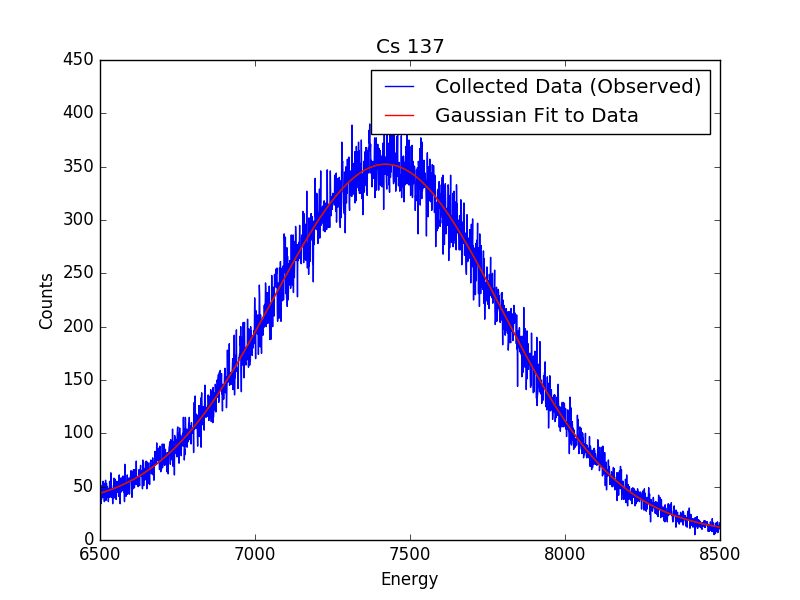
\includegraphics[width=\textwidth]{Cs137.png}
    \caption{Cs 137}
  \end{minipage}
  \hfill
  \begin{minipage}[b]{0.4\textwidth}
    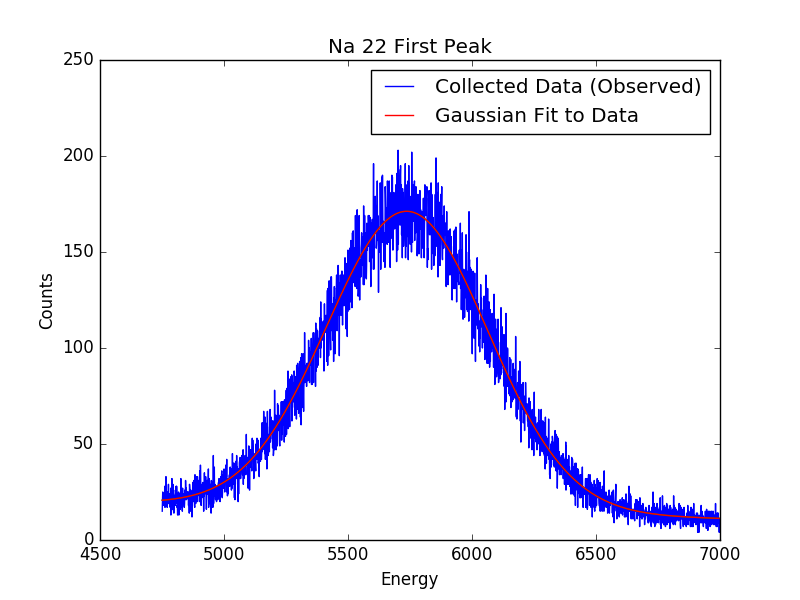
\includegraphics[width=\textwidth]{Na221.png}
    \caption{Na 22 First Peak}
  \end{minipage}
\end{figure}

\begin{figure}[H]
  \centering
  \begin{minipage}[b]{0.4\textwidth}
    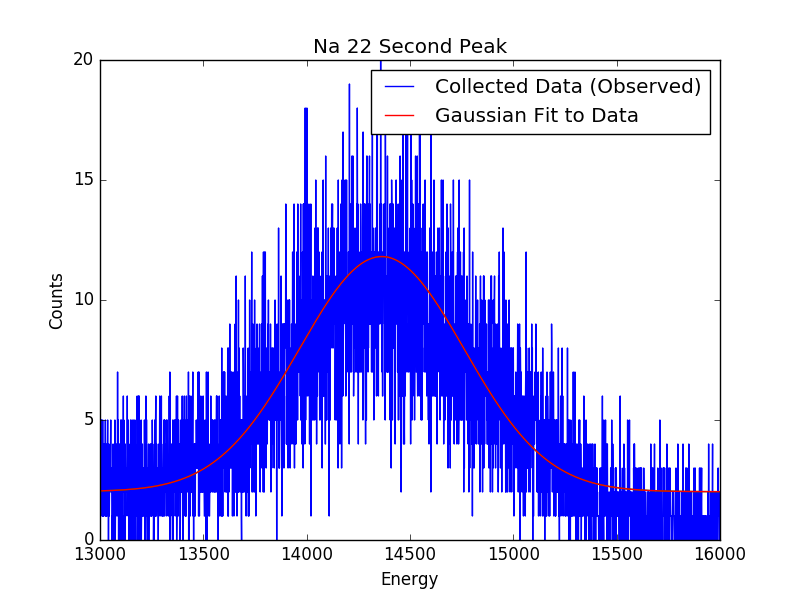
\includegraphics[width=\textwidth]{Na222.png}
    \caption{Na 22 Second Peak}
  \end{minipage}
  \hfill
  \begin{minipage}[b]{0.4\textwidth}
    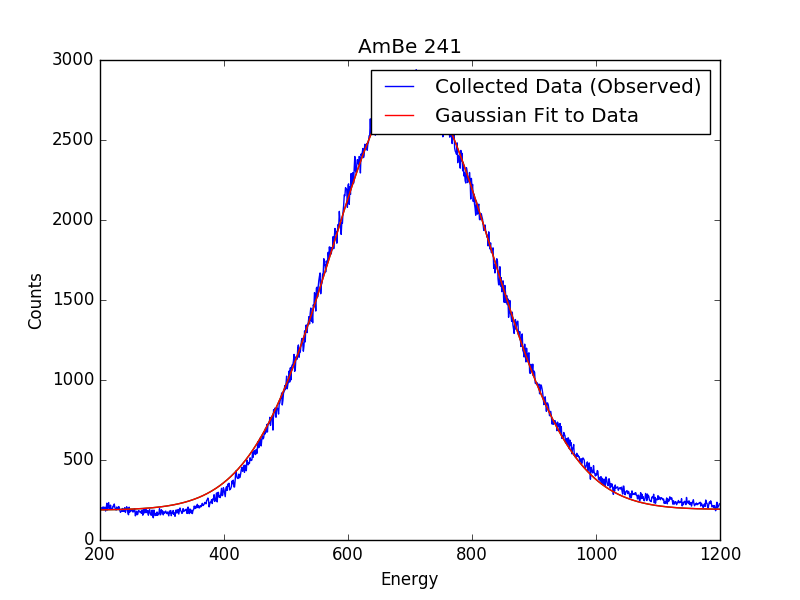
\includegraphics[width=\textwidth]{AmBe241.png}
    \caption{AmBe 241}
  \end{minipage}
\end{figure}


\begin{figure}[H]
  \centering
  \begin{minipage}[b]{0.4\textwidth}
    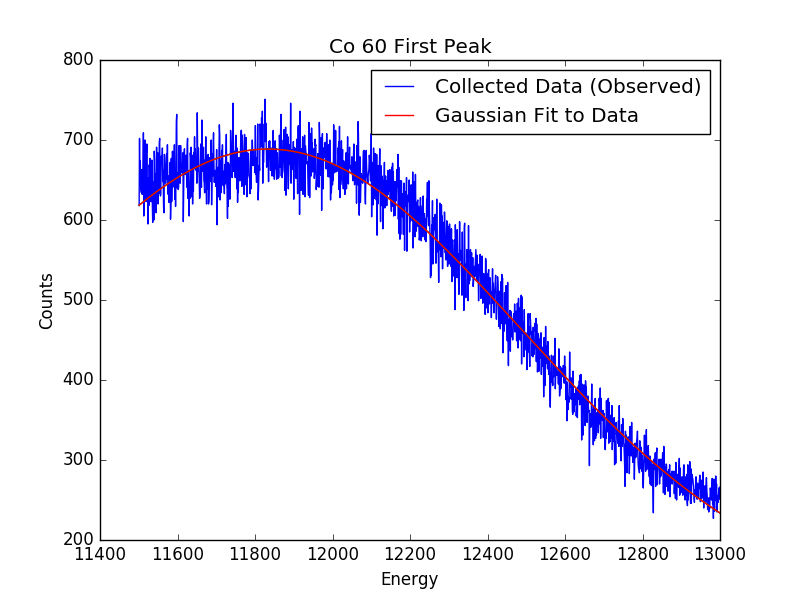
\includegraphics[width=\textwidth]{Co601.png}
    \caption{Co 60 First Peak}
  \end{minipage}
  \hfill
  \begin{minipage}[b]{0.4\textwidth}
    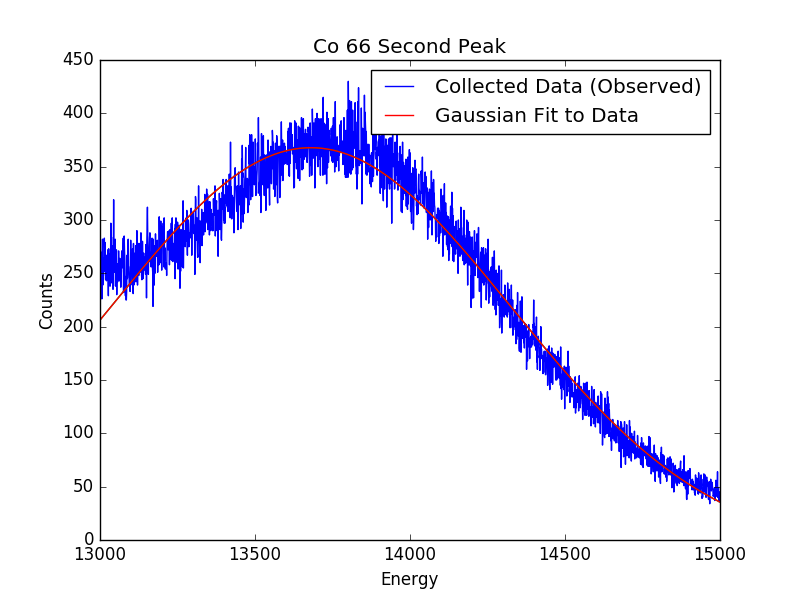
\includegraphics[width=\textwidth]{Co602.png}
    \caption{Co 60 Second Peak}
  \end{minipage}
\end{figure}

\begin{figure}[H]
  \centering
  \begin{minipage}[b]{0.4\textwidth}
    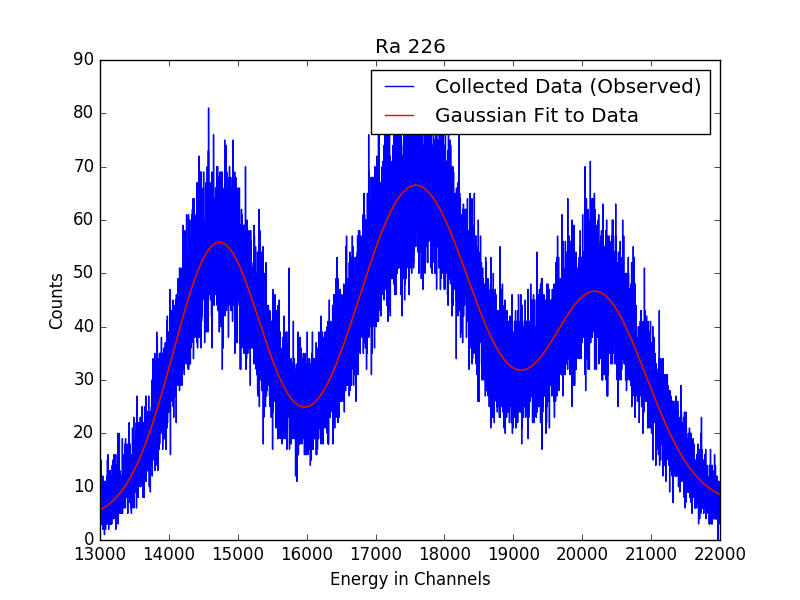
\includegraphics[width=\textwidth]{Ra1.png}
    \caption{Ra First Three Peaks}
  \end{minipage}
  \hfill
  \begin{minipage}[b]{0.4\textwidth}
    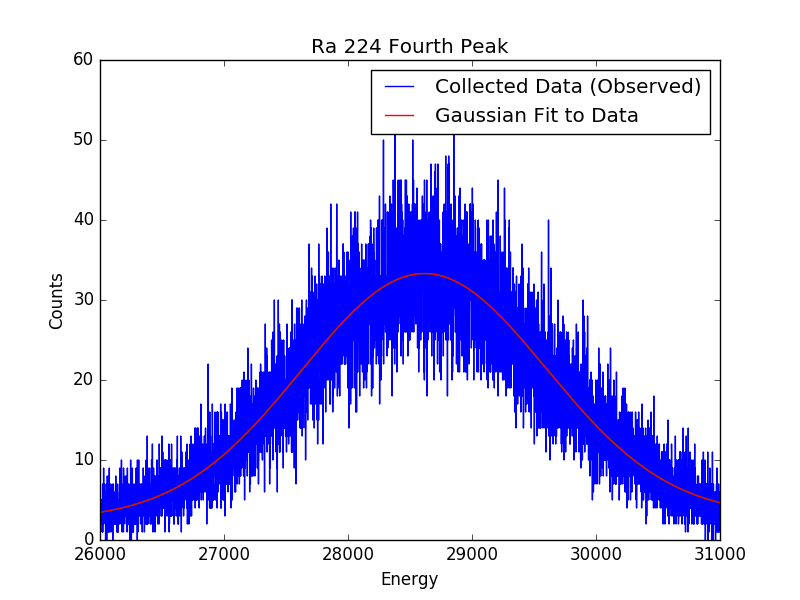
\includegraphics[width=\textwidth]{Ra4.png}
    \caption{Ra Fourth Peak}
  \end{minipage}
\end{figure}


After I had collected the data I used my scripts to create best fits for each source. I have attached each plot with the raw data and the fits plotted.Further analysis allowed me to plot a best-fit line of the channels to the known keV values; the slope of this line is 10.729 channels per keV [Figure 9]. Now all of the sources are gamma and electron decay, except the natural crystal impurity, which is an alpha source. The alpha sources do not convert from channels to expected keV values. The peaks are off by a factor ranging from 2.9 to 3.9 as a linear function of energy[Figure 10]. These values are the quenching factors for each alpha source and the linear fit is the quenching equation for an alpha source $ Quenching Factor = -0.00023*keV + 4.934$. 

\begin{figure}[H]
  \centering
  \begin{minipage}[b]{0.4\textwidth}
    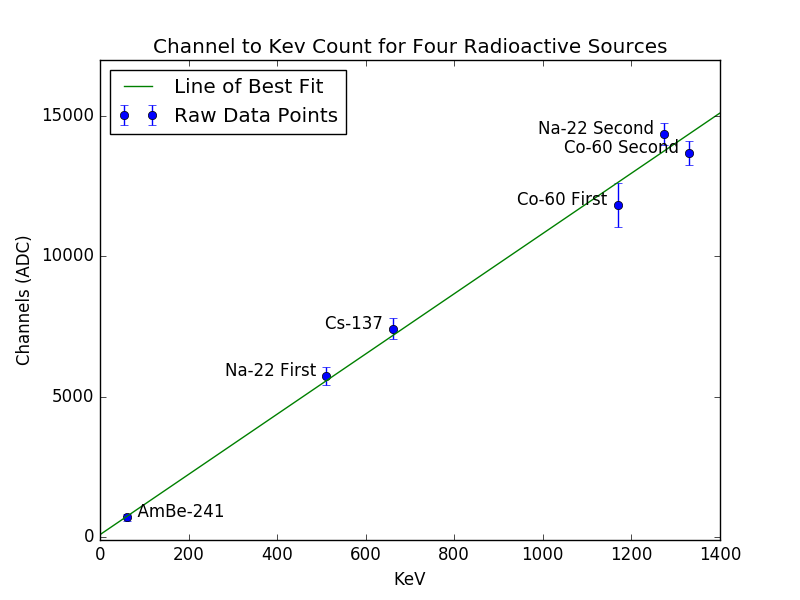
\includegraphics[width=1.4\textwidth]{ChantokeV.png}
    \caption{keV to Channel Linear Fit}
  \end{minipage}
  \hfill
  \begin{minipage}[b]{0.4\textwidth}
    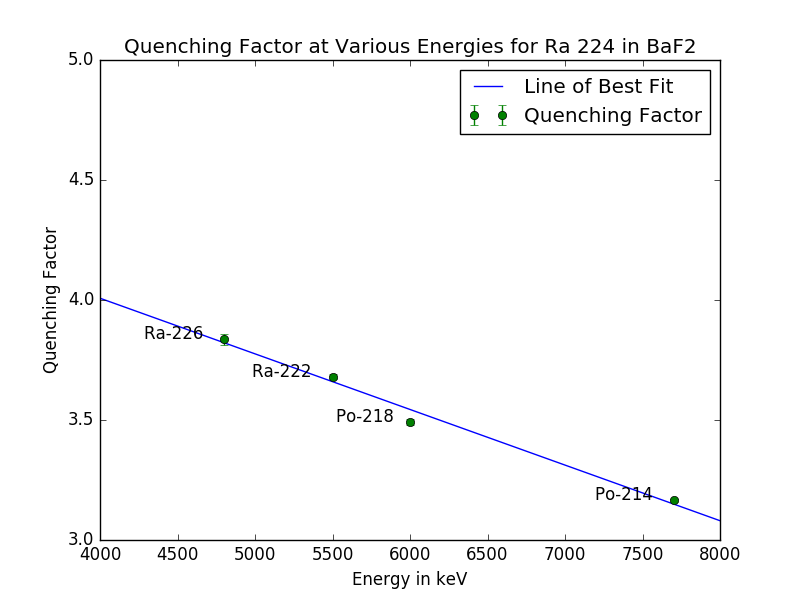
\includegraphics[width=1.4\textwidth]{QuenchingFactor.png}
    \caption{Quenching Factor from keV}
  \end{minipage}
\end{figure}

Lastly I plotted the slow and fast components of light through the Barium Fluoride crystal. Last year the SURF student in Professor Hitlin’s lab compiled the manufacturer’s data on the crystal. The manufacturer has determined the intensity of light received against the wavelength of the photon. The curves also reveal the slow and fast components of BaF2 scintillation. In the following figures the scatter plot values are shown as well as the Gaussian fit for the data [Figure 11].




\begin{wrapfigure}{r}{0.4\textwidth}
  \begin{center}
    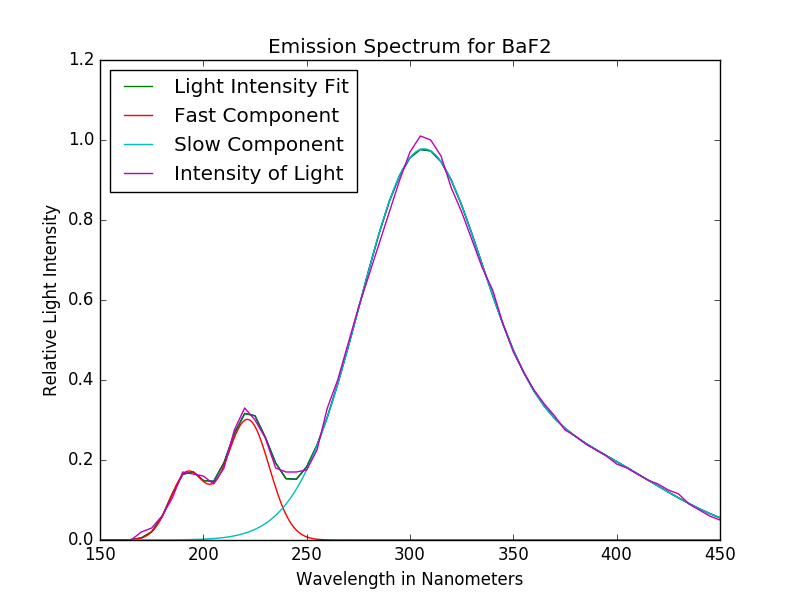
\includegraphics[width=0.6\textwidth]{FitsBaF2.png}
  \end{center}
  \caption{BaF2 Emission Spectrum Fits}
\end{wrapfigure}

In the next couple of weeks I will be repeating the experimental process I just completed for two other PMTs as well as the one I already tested. Each PMT can detect varying wavelengths of light and therefore represents the slow and fast components differently. I am repeating with the initial PMT with very strict collection protocol. I have discussed with the laboratory group and we have agreed the PMT will need to be left on, even when not in use, to maintain a stable temperature. This will keep the temperature constant to avoid variation affecting the results. I will also control for length of collection, distance the source is from the crystal, and the number of counts per channel. Once I have all of the sets I will use my refined and tested code to analyze all of the data. These fits and plots will be the ones used in the final research paper. 

The experimental values are in themselves useful to the field of particle physics. Reliable quenching factors for varying particles and PMTs will help research groups better understand their data for scintillation through BaF2. However little is known about the mechanisms that control the quenching factor. I will spend the rest of my SURF using my data and existing literature to analyze the physics behind Birk’s Law. I will work closely with a graduate student, Jake Kim, and my mentor, Professor Hitlin, for insight and explanation during this process. I will need to go further in depth in the literature of this field and explore with my mentors what is happening in more detail. Other than my limited exposure, I should have all of the tools necessary to complete my work. In addition to my project I will continue to learn about different experiments Hitlin’s group runs; a valuable part of my research exposure and SURF experience. Once I complete my experiments, data analysis, and analyzing the physics, I will begin compiling my results. I am on track to finalize these tasks and hopefully the group will be able to publish a paper with my findings in the near future.


\setlength{\parskip}{2em}
\noindent
Bibliography

\noindent
Birks, J.B. (1964). The Theory and Practice of Scintillation Counting. London:
Pergamon.

\noindent
Polischuk, O., Belli, P., Bernabei, R., Capella, F., Caracciolo, V., Cerulli, R., . . . Tretyak, V. (2009). Radioactive contamination of BaF2 crystal scintillator. Nuclear Institute.


\end{document} 









